%%%%%%%%%%%%%%%%%%%%%%%%%%%%%%%%%%%%%%%%%%%%%%%%%%%
%
%  New template code for TAMU Theses and Dissertations starting Fall 2016.
%
%
%  Original Author: Sean Zachary Roberson
%  This version adapted for URS by Parasol lab.
%  Adapted from version 3.16.10, which was last updated on 9/29/2016.
%  URS adaptation last updated 1/9/2017.
%
%%%%%%%%%%%%%%%%%%%%%%%%%%%%%%%%%%%%%%%%%%%%%%%%%%%
%%%%%%%%%%%%%%%%%%%%%%%%%%%%%%%%%%%%%%%%%%%%%%%%%%%%%%%%%%%%%%%%%%%%%%
%%                           SECTION III
%%%%%%%%%%%%%%%%%%%%%%%%%%%%%%%%%%%%%%%%%%%%%%%%%%%%%%%%%%%%%%%%%%%%%



\chapter{METHODS}

% In this chapter, we present the current problems with compatible item recommendation, and we provide a model aiming to solve these issues.

In this chapter, we present the problem of compatible item recommendation, and then, we present the design of our compatible item recommendation model.

\section{Problem Statement and Research Plan}
Given a set of items $I$ = $\{I_1, I_2, ... I_{|I|}\}$, we are trying to determine for each item $i$ in $I$ a set of compatible items $C_i$ = $\{ I_{c_1}, I_{c_2}, ... I_{|c_i|} \}$. Specifically, we are utilizing a large real-world dataset provided by Amazon introduced in \cite{mcauley-targett-shi-hengel} which features over a million products and 42 million co-purchased relationships across 20 top-level categories. We focus on the category of Cell Phone \& Accessories due to the prevalence of a variety of compatible characteristics. More specifically, we analyze all of the relationships between products in the top-level category of Cell Phone \& Accessories and their subcategories in order to find the compatible set $C_i$ for each product $i \in I$. We want to note here that although we are doing this analysis with just the Cell Phone \& Accessories category, this compatibility model can be applied to all top-level categories in the Amazon dataset. To accomplish our problem statement, we separate our solution into three parts: (i) define our definition of compatibility; (ii) classify each product with a specific product entity; (iii) utilize our compatibility classification to model complex compatible relationships.

\section{Defining Compatibility}

\begin{figure}[h!]
\begin{tabular}{ |p{6cm}|p{3cm}| }
 \hline
 \multicolumn{2}{|c|}{Sub-Category Compatibility} \\
 \hline
 Name & Type \\
 \hline
 Cases & Size \\
 Bluetooth Headsets & Interconnectivity \\
 Wired Headsets & Interconnectivity \\
 Chargers & Interconnectivity \\
 Cell Phone & Size \& Interconnectivity \\
 Screen Protectors & Size \\
 Internal Batteries & Size \& Interconnectivity \\
 External Battery Packs & Interconnectivity \\
 Battery Charger Cases & Size \& Interconnectivity \\
 Data Cables & Interconnectivity \\
 Smart Watches and Accessories & Interconnectivity \\
 \hline
\end{tabular}
\caption{Selected Cell Phone \& Accessories Sub-Categories and Type of Compatibility}
\end{figure}

In this section, we will define our definition of compatibility utilizing the type of relationships between top-level categories, their sub-categories, and the relationship within sub-categories. First, we organized each of the 20 top-level categories by their unique sub-categories and hand defined each sub-category's relation between each other and itself. For example, varying cases will be a size compatibility constraint, while varying chargers will be an interconnectivity compatibility constraint. Figure 3.1 describes this in more detail. There are some examples where size and interconnectivity both play a role in defining compatibility for a specific product. For example, the sub-category battery charger cases have both a size and interconnectivity component; the case has to be compatible with the size of the phone while the charger has to be compatible with the interconnectivity of the phone. While defining these relationships, we took caution to only consider the core functionality of the sub-categories, e.g. a case must be based on size and not fashion-sense. As a result, our definition of compatibility is derived from the relationship between sub-categories within top-level categories and comes in two forms: size and interconnectivity, for a specific product.

\subsection{Size}
As part of our definition of compatibility, we define size compatibility as the relationship between product $x$ and product $y$ such that $x$ and $y$ are strictly related to each other based on their physical appearance and dimensions while requiring that $x$ and $y$ both have the same top-level category. However, that means that $x$ and $y$ do not necessarily have to be in the same sub-category. In fact, it is crucial that $x$ and $y$ are in differing sub-categories for compatibility to be apparent. For example, an iPhone 4 and an iPhone 4 case belongs to the same Cell Phone \& Accessories top-level category. However, an iPhone 4 Case may belong to the sub-category of Cases, while an iPhone 4 may belong to the sub-category of Cell Phone. Therefore, the iPhone 4 and iPhone 4 Case have a size compatibility relationship. However, because an iPhone 4 and an iPhone 4s are both classified under the same sub-category of Cell Phone, they are not size compatible with one another.

\subsection{Interconnectivity}
Furthermore, we define interconnectivity compatibility as the relationship between product $x$ and product $y$ such that $x$ and $y$ are strictly related to each other based on their potential connectivity with each other while still requiring that $x$ and $y$ both have the same top-level category. However,there are many products in the same sub-category as $x$ that may not be interconnectivity compatible with $y$. For example, an iPhone 4 charging cable belongs to the sub-category of Data Cables in Cell Phone \& Accessories and has an interconnectivity compatibility relationship with the iPhone 4 in the Cell Phone sub-category in Cell Phone \& Accessories, but an iPhone 7 in the same Cell Phone sub-category in Cell Phone \& Accessories is not interconnectivity compatible with the same charging cable. To solve this, we develop a product entity classification that utilizes a natural language platform and our classification schema to build relationships between interconnectivity compatible products.

\section{Product Entity Classification}
\begin{figure}[h!]
    \begin{tabular}{ |p{0.5cm}|p{5cm}|p{4cm}|p{3cm}| }
     \hline
     \multicolumn{4}{|c|}{Sample Products} \\
     \hline
      & Name & Category & Entity \\
     \hline
     1 & Apple iPhone 4 AT\&T 16GB White & Cell Phone \& Accessories > Cell Phone  & Apple iPhone 4 \\
     2 & iPhone 4 Hello Kitty Case & Cell Phone \& Accessories > Cases & Apple iPhone 4 \\
     3 & Samsung S3 USB Cable & Cell Phone \& Accessories > Cables & Samsung Galaxy S3 \\
     \hline
    \end{tabular}
    \caption{Sample Products and their entity classification. The symbol '>' denotes a subcategory relationship.}
\end{figure}

After the classification of size and interconnectivity of sub-categories within top-level categories, we strengthen our definition of compatibility by classifying each product in each of these sub-categories with an entity. This entity will allow us to build our compatibility model and decide which products are compatible with other products. 

In Figure 3.2, we see sample products with their respective entity classifications. These classifications are necessary to decide size and interconnectivity compatible items. For example, product 1 belongs to the sub-category of Cell Phone while product 3 belongs to the sub-category of Cables. These items would be considered compatible if not for the interconnectivity compatibility definition. However, because these entities are different, we classify that product 1 and product 3 are not compatible. As another example, consider product 1 and product 2. Product 1 and product 2 belong in different sub-categories under the same top-level category Cell Phone \& Accessories. However, their entities are identical, classifying product 1 and product 2 to be compatible with each other. Our classification schema classifies over 340,000 products in this manner.


\subsection{Product Entity Classification}
In order to derive the product entity information, we utilized a natural language processing platform along with our classification model to recognize different entities of each product. After analyzing the benefits of multiple services, such as IBM Watson and Microsoft Cognitive Services, we decided to leverage the Google Cloud Natural Language Platform (GCL) due to the platform's ease of use, rapid response time, and consistent results. First, we analyzed the title and description of each product and queried GCL with this result. GCL then classifies each of the products into multiple entities based on product resemblance. Entities that GCL were able to classify include CONSUMER GOOD, ORGANIZATION, PERSON, LOCATION, EVENT, and etc. We used these entities, specifically CONSUMER GOOD, to decide what type of product the queried product was. In our case, CONSUMER GOOD was the only entity that described products that were purchasable objects. Using this entity, we found multiple amounts of CONSUMER GOOD entities for each product. To be more accurate in our classification, we decided to find the CONSUMER GOOD entity with the highest salience or accuracy percentage. In this way, we are able to be more accurate with our product entity classification model in analyzing what each product actually is and what items are compatible with each product. This CONSUMER GOOD entity corresponds to the entity that is in Figure 3.2.

We mapped each product to its highest CONSUMER GOOD salient entity. With this information, we created the product entity mapping for each product. 

\section{Compatibility Classification}
\begin{figure}[h!]
	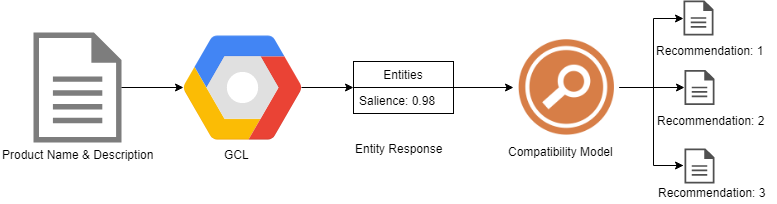
\includegraphics[scale=0.5]{data/Diagram.png}
	\caption{Item compatible recommendation work flow.}
\end{figure}

Utilizing the mapped product data in conjunction with the sub-category classification, we designed a compatibility classification model as follows. Each product has an entity mapping created by our classification model along with GCL. With this entity mapping, we are able to analyze compatible products, which are products that share the same entity but are in different sub-categories with the same top-level category. These are the items we would recommend the user. 

New products seeking compatibility recommendations are passed through GCL by title and description to get specific entities for that product. From there, the highest CONSUMER GOOD salient entity is gathered from the list of entities and is matched to our model to find other products that are compatible with the same CONSUMER GOOD salient entity. Next, we leverage all of the other sub-categories under the same top-level category of each item that is analyzed with the matching CONSUMER GOOD salient entity. From there, we return a subset of items from each sub-category as compatible items based on interconnectivity and size. Figure 3.3 shows a pictorial representation of our model and work flow. In this way, a variety of products cross-sub-category is recommended to the user that is compatible with the original product.


% For example, an iPhone 4 in the Cell Phone \& Accessories top-level category is not size compatible with a case for a Samsung Galaxy S3 even though the top-level category is size compatible with the sub-category of cases. Therefore, we must determine the entity in which each product is associated with. For example, the product 'Apple iPhone 4 AT&T 16GB White' belongs to Cell Phone \& Accessories and the product 'iPhone 4 Hello Kitty Case' belongs to the sub-category of Cases.


% For example, a product with title 'Apple iPhone 4 AT&T 16GB White' and 'iPhone 4 Hello Kitty Case' both belong to the entity of 'iPhone 4' are therefore are compatible. 


% Therefore, at the core of our research is the definition of compatibility. The difficulty arises from the novelty of the problem. Current recommender systems utilize collaborative filtering or content based recommendations as a metric for their recommendations. Compatibility is a human notion and therefore  


% \indent  Defining a new definition of compatibility is our biggest problem. This may be difficult because we have to research about what it means for something to be compatible by nature. Once we have figured out that definition, another challenge is to find ways of evaluating this new definition. This is a challenge because current evaluations of recommender systems use collaborative filtering efforts based on social-based recommendations. However, because ours is not of this form, we will have to devise new ways of implementing this. Finally, our last challenge is to define features that we will use to test this new definition of compatibility. We are proposing to test a range of electronics so that we can understand which electronics may be the most compatible with one another and if compatibility is really the best way of recommending electronics to users.

% \indent Another main challenge to note here is the cold start problem. The cold start problem is the problem that occurs when a new product is introduced. Because traditional recommender systems recommend compatible items based on co-purchasing, this new product has a very low chance of having any recommendations associated with it. This new product also has a very low chance of being recommended from other product selections. Our definition will solve the cold start problem by not relying on co-purchasing of items and instead focusing on text recognition and categories from the dataset to create a new definition of compatibility. Cold start problem doesn't affect how we determined annd defined our definition of compatibility.

% To accomplish this problem statement, we separate our solution into two parts. The first part is the text recognition platform, and the second part is the compatibility classification that we designed that contributes to our new definition of compatibility.

% \section{Method}

% \indent We first started by developing an idea about compatibility. In more depth, we wanted to see which products were compatible with other products. We searched through the Amazon dataset sorted by categories, and we created various documents based on the compatibility relationship between products in the same categories.  As a result, we developed a new notion - compatibility comes in two forms: size and interconnectivity.

% \subsection{Size}
% \indent As part of our definition of compatibility, we define size compatibility as products that fit together based on their physical appearance and dimensions. For example, an iPhone 4 is compatible with an iPhone 4 case but not an iPhone 7 case. Another example could be socks that are compatible with certain shoes based on shoe size.

% \subsection{Interconnectivity}
% \indent We define interconnectivity within our definition of compatibility as products that are compatible based on their connection with each other. For example, an iPhone 4 is compatible with an iPhone 4 charger, but an iPhone 7 is not compatible with this same iPhone 4 charger. Another example is a Macbook that is compatible with a traditional MagSafe Macbook charger but is not compatible with a Dell laptop charger.

% \indent To create this new definition of compatibility between items with these two classifications, we broke our solution down into two separate parts. The first part is the natural language platform that we used to recognize text and description of products, and the second part is the compatibility classification that we designed.

% \subsection{Natural Language Platform}
% \indent The text recognition platform that we have decided to use in conjunction with our compatibility model is the Google Cloud Natural Language Platform, otherwise known as GCL. We will use GCL to classify the text and description for each of the products in our dataset. This will allow our model to decide what kinds of products we are receiving from the dataset. Using this text recognition platform, we are to classify the overall key phrase for products in the same category. The natural language platform that we have decided to use in conjunction with our compatibility model is the Google Cloud Natural Language Platform. We will use the Google Cloud Natural Language Platform with our own model to classify the text and description for each of the products in our dataset. This will allow our model to decide what kinds of products we are receiving from the dataset. 

% \subsection{Compatibility Classification}
% \indent The compatibility classification model that we have designed is as follows. We take parts of the text-recognition classification. In particular, we are looking at the product with the highest salience in the consumer good entity. This is so that we can compare and contrast different consumer good entities to find out which of these products are compatible. If they share the same consumer good entity, then there is a higher probability that they are indeed compatible. However, an issue arises if they are the same or similar products. In this case, these products are not compatible. To solve this issue, we introduce the concept of categories. Using this natural language platform, we analyzed over 340,000 products and developed a classification schema that classifies each product in the dataset with key phrases that will contribute to the compatibility of that product based on the two notions of size and interconnectivity. We then develop relationship mappings between all products in the Amazon dataset based on our classifiers. After completion of this new definition of compatibility, if a user queries a product, our definition returns compatible recommendations for the user to choose and favorite. 


% \indent In our Amazon dataset, each product is labeled with categories and subcategories in which they belong in. For example, an iPhone case belongs in the category `Cell Phone & Accessories' and a subcategory `Cases'. Therefore, we can check compatibility by checking the categories of each of these products with the same consumer good classifier. If these categories are the same, then these products are classified as `similar' items and should not be compatible or recommended as compatible. If these categories are different, then this means that they are compatible in some shape or form. Therefore, we will recommend at least one product from each of the different categories in the same overall category. In this way, a variety of products cross-sub-category can be recommended to the user. 

% \indent We will introduce variables in both the natural language platform and the Amazon dataset. Figure 3.1 and 3.2 represent the variables for the corresponding models.

% The natural language platform has many variables, including... However, for the purposes of our research, we will only be looking at the salience value of the highest consumer good entity that we find in the platform classification as well as the name of the consumer good classifier. 

% The Amazon dataset also has many variables, including... However, for the purposes of our research, we will only be looking at the product name, description, categories, and also-bought items. 

% We will now discuss what these variables will be used for.



% %Fix table labeling.
% \begin{table}[h!]
% 	\centering
% 	\caption{San Japan attendance. Data is taken from \cite{ANCONS}. I intentionally make the title of this table long so the single space effect is seen in the list of tables.}
%         \vspace{1em}
% 	\begin{tabular}{|l|l|}
% 		\hline
% 		Dates & Attendance  \\ \hline
% 		August 8-10, 2008 & 3,523  \\ \hline
% 		August 14-16, 2009 & 4,003 \\ \hline
% 		July 9-11, 2010 & 5,049 \\ \hline
% 		August 5-7, 2011 & 6,891  \\ \hline
% 		August 10-12, 2012 & 9,464  \\ \hline
% 		August 16-18, 2013 & 11,077  \\ \hline
% 		July 18-20, 2014 & 14,686 \\ \hline
% 		July 31-August 2, 2015 & 18,411  \\ \hline
% 	\end{tabular}
% \end{table}

% You may be wondering why San Japan was chosen. There are a few reasons as to why I did this:

% \begin{enumerate}
% \item It is one of the fastest-growing anime conventions in Texas.
% \item Filler.
% \item I wanted a good variety of table examples.
% \item Because conventions are cool.
% \end{enumerate}

% The \textit{enumerate} environment was used to generated an ordered list above.

% \section{Section Test Example}
% We insert another figure here, just for kicks.

% \begin{figure}[h!]
% 	\centering
% 	\includegraphics[scale=0.5]{LowPass_Filter_Design.png}
% 	\caption{A low pass filter design.}
% \end{figure}

